\documentclass[12pt]{article}
\usepackage[utf8]{inputenc}
\usepackage[T1]{fontenc}
\usepackage{unicode-math}
\newcommand{\EE}{\mathbb{E}}
\newcommand{\R}{\mathbb{R}}
\usepackage{amsmath,amsfonts,amssymb}
\usepackage{graphicx}
\usepackage{a4wide}
\bibliographystyle{unsrt}
\usepackage{biblatex}
\usepackage{import}
\bibliography{draft.bib}


% Comments for co-authors (optional)
\newcommand{\coauthorcomment}[2]{{\color{#1} \textbf{#2}}}

% Title and author information
\title{Sign operator for $(L_0, L_1)$-smooth optimization}

\author{
  Mark Ikonnikov\\
  \texttt{ikonnikov.mi@phystech.edu}
  \and
  Nikita Kornilov\\
  \texttt{kornilov.nm@phystech.edu}
}

\date{\today}

\begin{document}
\maketitle


\begin{abstract}
In Machine Learning, the non-smoothness of optimization problems, the high cost of communicating gradients between workers, and severely corrupted data during training necessitate generalized optimization approaches. This paper explores the efficacy of sign-based methods~\cite{pmlr-v80-bernstein18a}, which address slow transmission by communicating only the sign of each minibatch stochastic gradient. We investigate these methods within $(L_0, L_1)$-smooth problems~\cite{gorbunov}, which encompass a wider range of problems than the $L$-smoothness assumption. Furthermore, under the assumptions above, we investigate techniques to handle heavy-tailed noise~\cite{Kornilov2025}, defined as noise with bounded $\kappa$-th moment $\kappa \in (1,2]$. This includes the use of SignSGD with Majority Voting in the case of symmetric noise. We then attempt to extend the findings to convex cases using error feedback~\cite{karimireddy}.
\end{abstract}

\paragraph{Keywords:} Sign-based methods, $(L_0, L_1)$-smoothness, high-probability convergence, heavy-tailed noise.

\paragraph{ Highlights below to be fixed later (these are our hopes for the paper)}

\paragraph{ Highlights:}
\begin{enumerate}
\item Proves convergence of sign-based methods for $(L_0, L_1)$-smooth optimization
\item Handles heavy-tailed noise with high-probability convergence guarantees
\item Extends sign-based optimization to convex functions using error feedback
\end{enumerate}

\section{Introduction}


\import{./}{intro}


\section{Computational experiment}

\section*{THIS PART WILL BE DELETED}

\begin{figure}[!h]
    \centering
    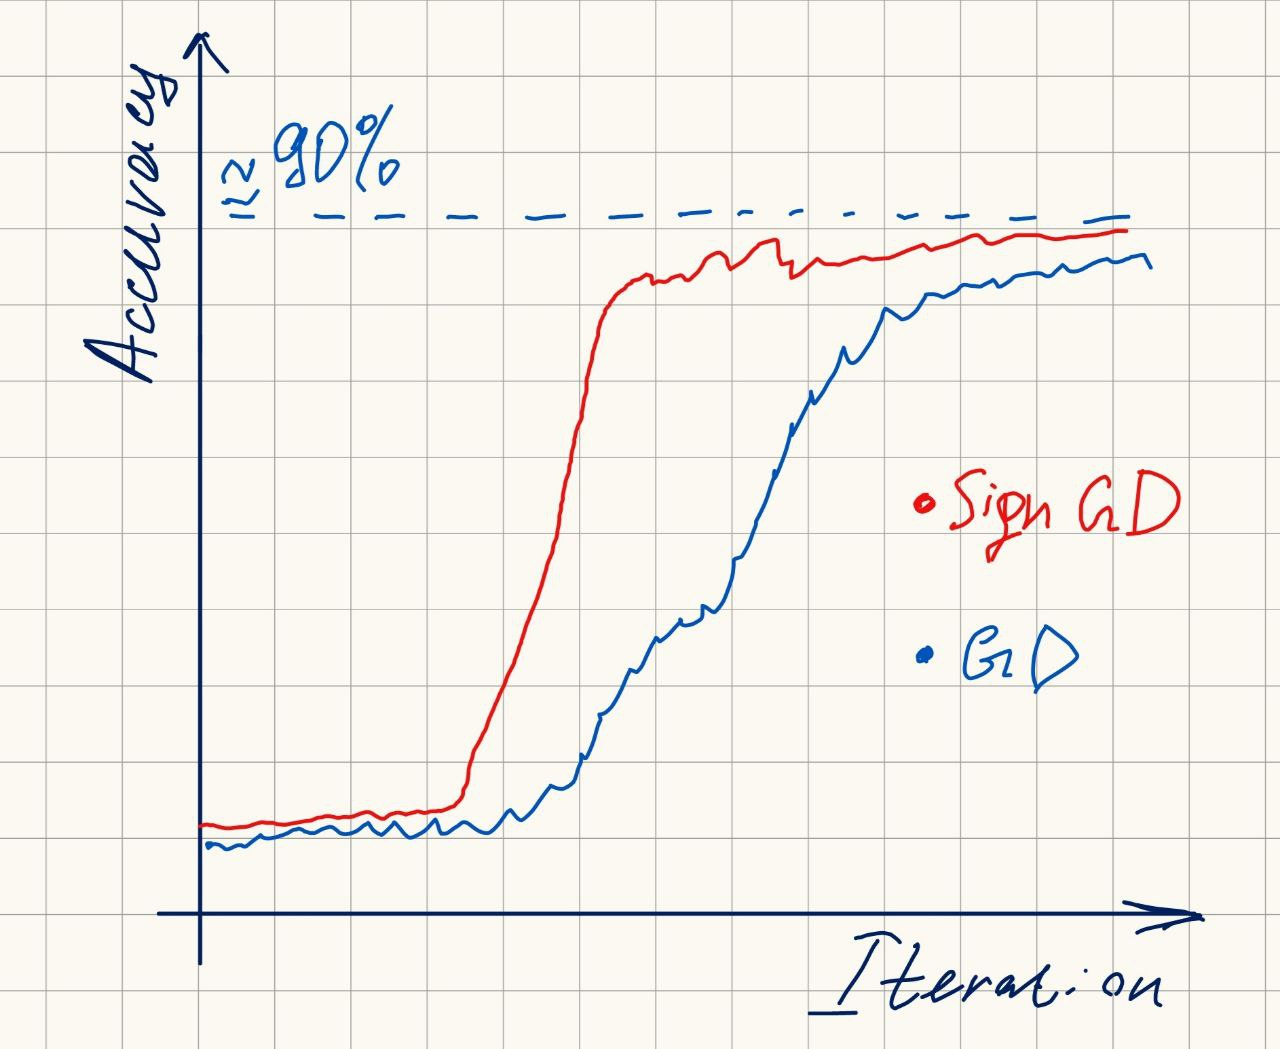
\includegraphics[width=0.3\textwidth]{drawing.jpg}
    \caption{Performance of GD, SignGD}
    \label{fig:logreg}
\end{figure}

The computational experiment aims to compare the performance of standard gradient descent (GD) and sign-based gradient descent (Sign-GD) in training a logistic regression model, highlighting the advantages of sign-based methods under L0 and L1 smoothness assumptions. Performance will be evaluated based on accuracy and iteration number, with minimal tuning to emphasize simplicity.

The experiment compares standard gradient descent (GD) and sign-based gradient descent (Sign-GD) on an open-source binary classification dataset "Mushrooms". Below is a mini-report based on expected outcomes.
The preliminary plot (hand-drawn) shows Sign-GD achieving comparable or better performance with faster convergence, consistent with $(L_0, L_1)$ smoothness assumptions.

Comments: 
The idea is based on the fact that logistic regression function $l(z,y) = \ln (1 + \exp(-yz)$  is both smooth and $(L_0, L_1)$-smooth, with $L = || y ||^2$ and $L_0 = 0, L_1 = || y ||$ which can be much smaller than $L$. Sign-GD slightly outperforms GD in accuracy and convergence time, suggesting that the sign-based update leverages smoothness assumptions effectively. The simplicity of the approach (no complex tuning) aligns with the minimal-effort goal. These results do not contradict the experiment’s aim to showcase sign-based method advantages.
\begin{figure}[!h]
    \centering
    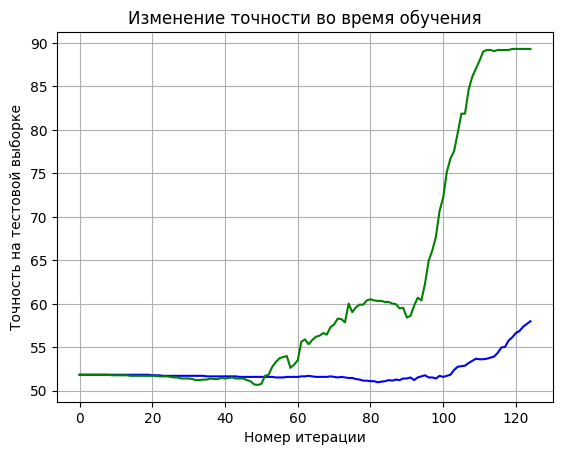
\includegraphics[width=0.9\textwidth]{basic_experiment.png}
    \caption{Logistic regression on Mushroom Dataset.\newline Performance of GD, SignGD with $L_1 $-tuned step size}
    \label{fig:logreg}
\end{figure}




\newpage

\printbibliography

\end{document}